\documentclass[11pt]{article}

\usepackage{sectsty}
\usepackage{graphicx}
\graphicspath{ {./images/} }
\usepackage{indentfirst}
\usepackage{subcaption}

% Margins
\topmargin=-0.45in
\evensidemargin=0in
\oddsidemargin=0in
\textwidth=6.5in
\textheight=9.0in
\headsep=0.25in

\title{ Son Görüşmeden Sonra Olan Kısımların Raporu}
\author{ Özgür Temmuz Çelik }
\date{\today}

\begin{document}

\pagebreak

\centerline{\large \textsl{ EE492 Senior Project} }
\vskip 5mm

\vspace*{3cm}
\centerline{\Large \bf  Scene Recognition with Federated Learning }
\vskip 2cm

\centerline{\large\bf  Özgür Temmuz Çelik} 
%\vspace*{2mm}   
%\centerline{\large\bf  Project-PartnerName} 

\vspace*{2cm}
\begin{center}
{\large\rm  Department of Electrical and Electronic Engineering}
\end{center}

\vskip 2cm
\begin{center}
{\large\rm  Project Advisor:  H.~I\d{s}{\i}l~Bozma}
\end{center}  

\vspace*{2cm}
\begin{center}
\today \\[2cm]
{Bo\u{g}azi\c{c}i University}\\[5mm]
{\large\rm      Bebek, Istanbul 34342} \\
\end{center}
%\vspace*{20mm}

\newpage

\begin{abstract}

\par We present a federated learning approach to scene recognition task where the dataset is distributed to the agents/clients in a highly heterogenous manner. Our goal is to ensure agents can learn recognizing all the scenes even if they have no data samples from some of the scenes. While doing that we also adhere to a strict privacy constraint of not sharing data samples between agents. We also investigate the fast adaptation to novel places and scenes when a backbone is trained with federated learning.

\end{abstract}

\newpage

% Optional TOC
\tableofcontents
\pagebreak

%--Paper--


\listoffigures
\pagebreak

\section{Introduction}
With the advancement of technology some resource intensive tasks of the past like data collection and machine learning training can now be realized by the edge devices like cellphones, wearable products such as like smart-watches, stationary cameras with some IT support and ever more popular robots. This advancement has also brought upon a new emphasis on data privacy and security. Federated learning \cite{originalFL} is a new distributed learning methodology that trains a machine learning model across multiple clients, decentralized devices, holding their own local data and provides privacy on learning by only sharing model parameters rather than the data with the centralized server. In general, federated loss we want to minimize is the average of client losses.

\begin{equation}
f(w) = \frac{1}{n} \sum_{i=1}^{n} f_{i}(w)
\end{equation}

with $f_{i}(w)$ being the loss of the prediction on a sample $(x_i,y_i)$ given model parameters $w$, $f_{i}(w) = l(x_i,y_i;w)$. $n$ is the number of clients sampled at that particular epoch. As one can infer not necessarily every client takes part in every epoch. At each training epoch central model is broadcasted to the clients, each client trains for a given number of rounds on its own local data, and finally the gradients of client models are aggregated to the central server where the central model is updated using federated averaging. In this project our goal is to apply federated learning to scene recognition tasks modelling intelligent agents gathering data samples from different scenes and places and trying to learn not only from their own dataset but from the datasets of other agents without sharing data samples. In short, we hope to use federated learning to ensure information sharing with strict privacy constraints. In Chapter 1, we have setup our test to distinguish between different scenes. In Chapter 2, we went a step further and investigated distinguishing not only places from different scenes but from the same scene: for example classifying 2 offices among other places from different scenes. In that chapter, we also extended our work to fast adapting to novel scenes and places that no client has seen before by using a transfer learning technique.


\section{Chapter 1}

\subsection{The Model and Dataset}

\par In our tests we have used the raw image data of “Stanford 2D-3D-Semantics Dataset” \cite{stanfordDataset}.  We have divided our dataset to 6 clients as it was suggested in \cite{stanfordDataset}. How did we handle the actual data distribution? For IID case we have randomly assigned data samples but for non-IID case we have used a dirichlet parameter-based data distribution \cite{dirichlet}. This data distribution can be seen at Figure \ref{fig:distSmall}. The x axis shows the classes/scenes of which we have eleven, and the y axis shows what percentage of this class belongs to a given client. For example, take class 7, it is completely divided between 2 clients and other 4 clients have no samples of it. As we can see our non-IID distribution is highly heterogenous. By using such a heterogeneous data distribution, we want to know if a client can learn a class that it has no samples of. If we turn back to class 7 example, 4 clients have no samples from that class so if we manage to classify this class reliably then we can conclude those 4 clients have learnt to classify this class despite not seeing it at all. This is why we are investigating a federated learning approach to intelligent agent questions.

\begin{figure}[h!]
\centering
  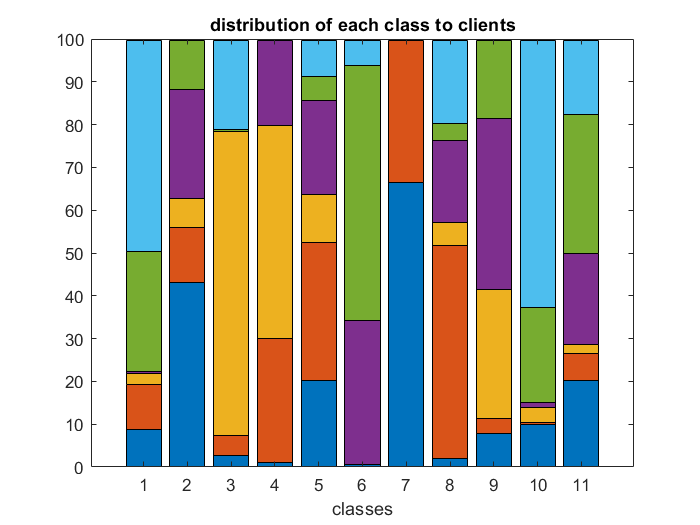
\includegraphics[scale=0.5]{distSmall}
  \caption{Non-IID Data Distribution}
  \label{fig:distSmall}
\end{figure}

\par It must be noted even the raw image part of the original dataset is very large (64 GB) since it uses 1080x1080 images. Using the original dataset as is would be unfeasible so to create our dataset, we have used 64x64 images. As our model we used the model proposed in the original federated learning paper \cite{originalFL}. The basis of this model is convolutional layer followed by max pooling layer. We have two such combination. Max pooling is done over a 2by2 windows which means the height and width of channels are halved each time. The first convolutional layer takes 3 channels (RGB) and returns 32 channels whereas the second convolutional layer takes 32 channels and return 64 channels. These layers are followed by a dense layer of size 512 which leads to 11 outputs. As we can see our model is quite simplistic by today’s standards. When it comes to training, we have run our tests for 500 rounds to see them to converge. We are not only interested in the path accuracy plots follow but also the eventual accuracy they settle to. We have used SGD with 0.01 learning rate and 0.9 momentum in all of our tests in this chapter.

\subsection{Client Participation}

\begin{figure}[h!]
\centering
  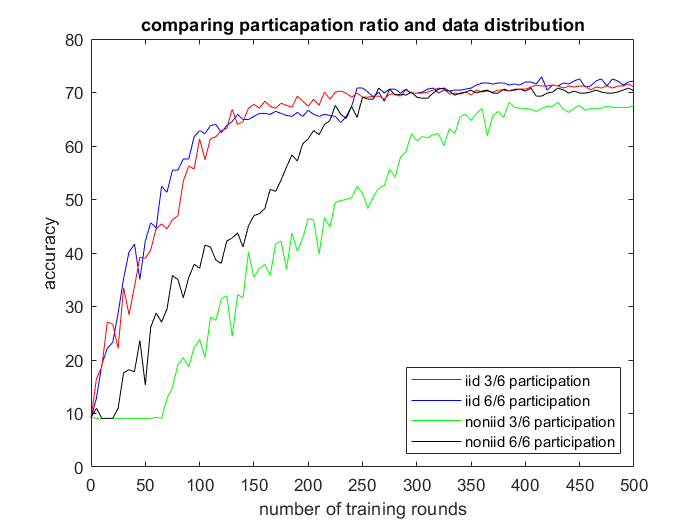
\includegraphics[scale=0.5]{ratioIIDvsNonIID}
  \caption{Effects of Client Participation}
  \label{fig:clientSelection}
\end{figure}

We first wanted to investigate the effects of client selection and non-IID data distribution. There are multiple techniques \cite{clientSelection1}\cite{clientSelection2} developed for biased client selection for heterogenous data distributions in which the odds of choosing a specific client for training is either increased or decreased, but these techniques require us to know the data distribution at clients apriori or show preference to some clients on the fly. For that reason, the most common client selection technique is unbiased or random client selection. This unbiased client selection can be used to reduce the total communication cost -note that per client communication cost stays same- or it can be used as a very simplistic model of effects of client availability. To achieve these goals, we have run 4 tests. These tests are combination of IID vs non-IID data and 6/6 client participation vs 3/6 client participation. Now looking at our results at Figure \ref{fig:clientSelection} we can clearly see when we are using IID data, halving the participation ratio doesn’t negatively affect our accuracy. Both accuracy plots follow the same path and converge at same training rounds. Comparing the IID 6 client participation and non-IID 6 client participation we can clearly see the adverse effects of non-IID data. Despite converging to same accuracy, for a long time there was a significant accuracy drop between the two. Additionally, it took roughly 50 training rounds for non-IID one to reach the same accuracy as IID one. When we use IID data distribution for federated learning for the most part all the clients converge in the same direction in every training round, so the cancellation when averaging is not common. But when we train with non-IID data distribution since all the clients have different local data distributions the cancellations are much more common. These discrepancies lead to server model getting trained more slowly and requiring more training rounds than it would be necessary otherwise. When looking at the IID data distribution we have said using 3 client participation instead of 6 doesn’t negatively affect the training, but it is obvious this observation doesn’t extend to non-IID data distribution. 3-client participation non-IID case not only significantly lagged the 6-client participation, but also it failed to converge to the same accuracy all the others did. This means no matter how long we train, if we are using 3-client participation, we will never reach to 6-client participation accuracy scores. Why did our performance suffer so badly when using 3-client participation was fine with IID data? We believe since our non-IID dataset is highly heterogeneous there are training round cases in which some scenes are not present at all or represented at low numbers that hinder the model training. Take scene 7 for example, all the samples of that scene are only present at 2 clients alone and if those clients are not chosen for training then our model not only doesn’t train on scene 7 but also forgets its past training. Given the fact that almost all of the scenes have at least half of their samples at two clients we can see how prevalent this problem is. We argue this is the main reason why for non-IID case less than full client participation has such detrimental effect.

\subsection{Encoding}

\begin{figure}[h!]
\centering
  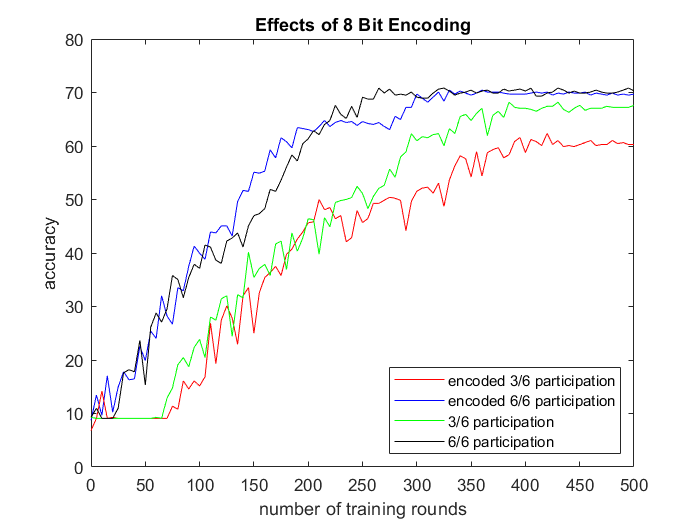
\includegraphics[scale=0.5]{encoding}
  \caption{Effects of 8-Bit Encoding}
  \label{fig:encoding}
\end{figure}

\par As we have mentioned in the client selection part it is desirable to reduce the communication costs of federated learning. The main way to do that is encoding \cite{compression1}\cite{compression2}. In the standard versions of federated learning it is customery to use 32 bit floating values, but do we really need all these 32 bits? Here we must note we are talking about communication only, so the image itself and the computations done at the clients and server are still using 32 bits. Also note we are not encoding all the gradient values. If a tensor is shorter than a threshold, in our case 10000, then we choose not to encode it since the gains will be small and encoding the final dense layers have detrimental effects on accuracy far overshadowing the gains\cite{compression2}. We wanted to test the effects of encoding and its relation to client participation ratio. Please note all the tests have been conducted using the non-IID data distribution given in \ref{fig:encoding}. When we look at the 6-client participation case we see encoding didn’t effect the accuracy plot much. The encoded case has managed to converge to the same accuracy original one did. But when we look at the 3-client participation case we see the encoded one failed to converge to the nonencoded 3-client’s accuracy- there is a near 7\% accuracy drop. Why did 3-client case suffer when 6-client case seems to be doing fine? We believe this can be explianed by treating the encoding as a bounded noise. First let’s discuss why this is the case. When we encode the 32 bits to 8 bits we are basically losing the information that 24 bits carried. The absolute value of this information has the same possiblty to be anywhere from zero to the maximum value we can represent with this 24 bits. Since we might have rounded the leading 8 bits up or down the lost information might be positive or negative. Now obviosuly this lost information is not gaussian distributed but for the sake of argument let’s treat it as AWGN and average it like we are doing in server. Assume the sample noise variance is $Var(z) = E[z^2] = \sigma^2$

\begin{equation}
Var(N_{avg}) = Var(\frac{1}{n}\sum_{i=1}^n z_i) = \frac{1}{n^2}
\sum_{i=1}^n Var(z_i) = \frac{1}{n^2}n\sigma^2 
	= \frac{1}{n}\sigma^2
\end{equation}

\par As we can see averaging signals with AWGN noise reduces the noise power by 1/N. So doubling our client number from 3 to 6 halves the power of AWGN. Of course we aren’t dealing with AWGN here and there is a randomness involved due to very nature of machine learning but we can see why increasing number of clients makes our system more robust to adverse effects of encoding. 

\par Using this 8-bit encoding our communication costs per client has been reduced from 329Mb to 95Mb. This means more than 70\% reduction in communication costs.

\subsection{Differential Privacy}

\begin{figure}[h!]
\centering
  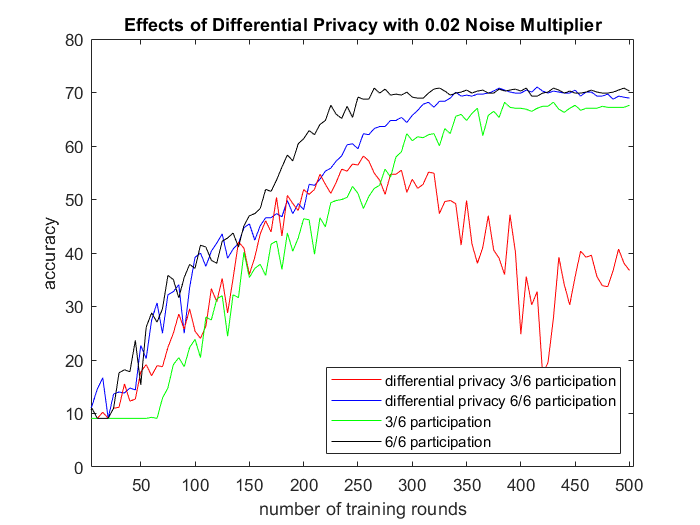
\includegraphics[scale=0.5]{diff}
  \caption{Effects of Differencial Privacy}
  \label{fig:diff}
\end{figure}

\par The big selling point of federated learning is data privacy. By training each client locally and never transmitting their data to server, federated learning offers a great level of privacy. But we are transmitting the server model to clients and then client gradients after local training to server and if somehow an attacker gains access to both server model and a client’s gradients then the attacker may reverse enginner data distribution of said client. How does that work? When attacker adds the gradients of client to the server model he/she gets the final version of client model at the end of local training. If attacker is aware of which classes are there in this domain then attacker can compare the results of both server model’s and the client model’s accuracies. If client model performed worse at some classes then those classes are likely not present in that client’s local dataset. Or if the client model performed significantly better at some classes then those classes are likely very prevalent in the client’s local dataset. This is a very simplistic example and the privacy leakeage usually happens in multiple communication rounds \cite{advancesAndOpenProblems} but we can see how this privacy leakeage can lead to problems.  One common technique to solve this problem is using encyription. Most common ones are homomorphic encyription \cite{HE} and secure multiparty computation \cite{SMC}. This methods make use of encyription methods we can do computations on encyripted values. 

\par Another method, a more simplistic one, is differential privacy \cite{diff1}\cite{diff2}. In differential privacy we basically introduce noise some multiplicant of the clipping of a tensor. We choose this method since this is by far the most prevelant one and it is fairly easy to use. In our tests we have used a noise multiplier of 0.02. For 6-client case, the accuracy plot closely follows the that of original and finally converges at the same ratio. When it comes to 3-client case we see that it diverges around 250 rounds and never recovers. At the end we see near 30\% accuracy drop and failure to convergence. Why did 6-client and 3-client cases differ so significantly? We once again use the AWGN modelling and argue the increase in the client number made the model more resilient to noise. But then why did encoding and differencial privacy plots differ so much? We have 2 reasons for that. First, the noise levels are not same. Second, in encoding we do not alter the final fully connected layer whereas in differential privacy we alter those.  

\section{Chapter 2}

\subsection{The Model and Dataset}

\par		In the last chapter we have shown, through federated learning, clients can learn recognizing scene categories that they have no samples of. Expanding on that we want to know whether we can learn not only different scene categories like office, pantry etc. but also different places among those categories. For example, can a client learn to differentiate between different offices some of which it may have never seen before?
\par		First, we had to decide how our dataset should be. Given the fact that recognizing inner-scene differences is a more challenging task than recognizing differences between scenes, we need a more robust feature extractor and higher quality images. We decided to use ResNet-18 -which is much deeper than the CNN architecture we used in the last chapter- accompanied by 160x160 images. When we look at the original Resnet-18 paper\cite{resnet18} we see that they have used 224x224 images and those images went through 5 halving in total -reduced to 1/32th of original size in each side- till they reach the average pooling layer as 7x7 channels. We believed using 224x224 images might be too computationally expensive, so we used 160x160 images which meant we had 5x5 channels at the average pooling stage. All this Resnet-18 architecture until the Fully Connected (FC) layer at the very end is called the feature extractor or backbone.

\begin{figure}[h!]
  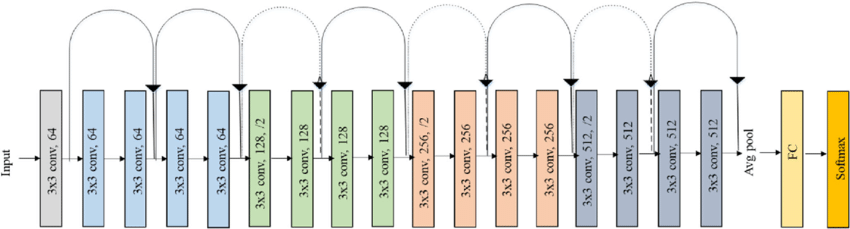
\includegraphics[scale=0.5]{resnet18}
  \caption{ResNet-18 Architecture}
  \label{fig:resnet18}
\end{figure}

\par Now that we have determined our model and the image sizes, we now must determine the size of the dataset. We decided to use 3 scene categories (office, lobby, hallway) with 3 places from each scene category so in total we have 9 classes/places. Places 1,2 and 3 are offices; 4,5, and 6 are lobbies; 7,8, and 9 are hallways. We picked 90 images randomly from each place and used 20\% of those as test set to measure accuracy and create confusion matrix. It should be noted that we didn’t pick those places randomly instead we made sure 90 images from a place were enough to have a good representation of that place. So, the places we took those 90 pictures from had around 100 to 200 images in total. This constraint excluded places from scenes like auditorium which had more than 2000 images each. It would be impossible to pick 90 images that could represent the feature space of such places adequately. 

\subsection{Central and Federated Learning Comparison}

\par Before moving on to federated learning we checked the model in a central machine learning setting to make sure the model-image properties are sufficient. At the end of this very standard machine learning training, we got the \ref{fig:centralanddist}{(a)} with 83\% overall accuracy.

\begin{figure}[h!]
  \centering
  \begin{subfigure}[b]{0.4\linewidth}
    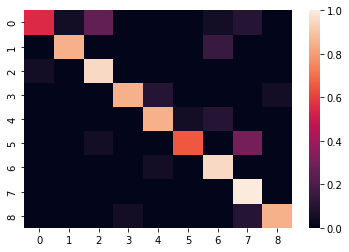
\includegraphics[width=\linewidth]{central.png}
    \caption{Confusion matrix of central training}
  \end{subfigure}
  \begin{subfigure}[b]{0.4\linewidth}
    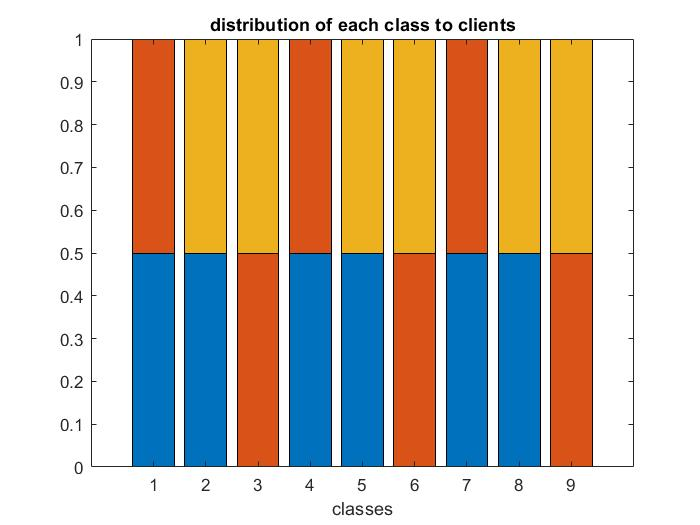
\includegraphics[width=\linewidth]{dist.jpg}
    \caption{Data distribution for federated learning}
  \end{subfigure}
  \caption{Central Training and New Heterogeneous Data Distribution}
  \label{fig:centralanddist}
\end{figure}

\par As we can see from the confusion matrix all the places except the first one separated very well and the samples from first one were sometimes predicted as yet another place of same scene category -office. It should be noted further accuracy improvements can be observed by training longer, but our goal was not to get the best central training result rather show our Resnet-18/160x160 image setting is adequate. We concluded the Resnet-18 using 160x160 images is robust enough to learn multiple places from multiple scenes. Moving on to the federated setting class distributions to clients can be found at \ref{fig:centralanddist}{(b)}. Here we have used 3 clients in total and this number was decided due to computational constraints. Each client has samples from 6 out of 9 places and each place is available at the dataset of 2 out of 3 clients. It is important to note while 2 different clients may have training samples from same place, the samples are not same/repeated; each of those two clients hold half of the samples of that place. Using the dataset and the distribution we have described, we run the federated averaging for 300 rounds with each client participating to each communication round.

\begin{figure}[h!]
  \centering
  \begin{subfigure}[b]{0.4\linewidth}
    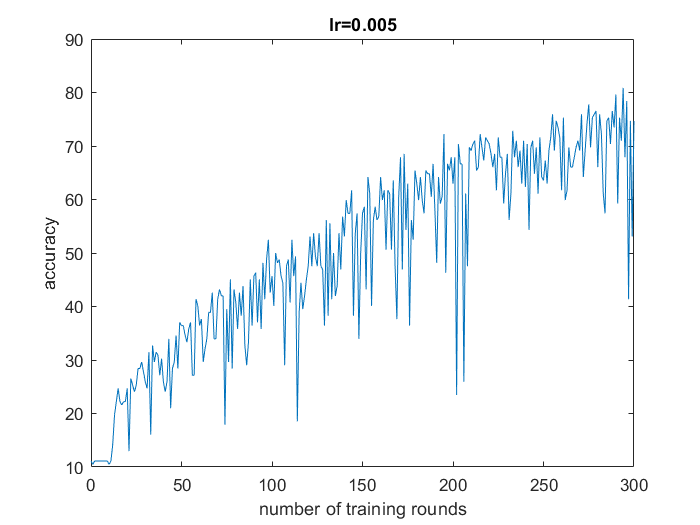
\includegraphics[width=\linewidth]{training.png}
    \caption{Accuracy plot}
  \end{subfigure}
  \begin{subfigure}[b]{0.45\linewidth}
    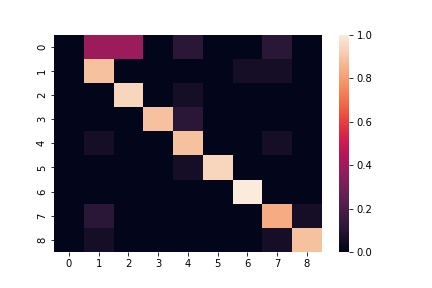
\includegraphics[width=\linewidth]{fedStanford901lr005.jpg}
    \caption{Confusion matrix for federated learning}
  \end{subfigure}
  \caption{Accuracy Plot and Confusion Matrix of Federated Learning}
  \label{fig:fedtraining}
\end{figure}

\par Looking at the \ref{fig:fedtraining}{(a)} accuracy plot, we can see our system is not very stable despite the fact accuracy kept improving when tracked over a long period. Why do we have sporadic dips? Looking at the last chapter we see that the simpler CNN architecture was much more stable. We speculate as the architecture gets deeper and deeper small differences can have larger overall effects and can cause dips in accuracy. This instability led us to use 0.005 learning rate for client optimizers (SGD). Beforehand we were using 0.01 but when we run our trial runs with that learning rate the instability was even worse and it was hindering accuracy improvements. Using a smaller learning rate enabled us to achieve somewhat steady accuracy improvement. At the end of the 300 rounds, we have achieved 76\% accuracy. Looking at the \ref{fig:fedtraining}{(b)} confusion matrix we see that all the places except the first one has separated very nicely. First one was almost always predicted as second and third places which are from the same scene as the first one -offices. This is a very promising result since it implies the model has learned features of a place are most similar to the features of places from the same scene. Also, we should remember the first place was already the worst performing one in central training.

\subsection{Generalization to Novel Scenes and Places}

\par An open problem in federated learning is generalization to novel clients \cite{advancesAndOpenProblems}. Taking inspiration from transfer learning and personalized federated learning via layer sharing \cite{layerSharing} we decided to check if the feature extractor we got by federated learning is capable of extracting the features of novel places well enough to distinguish between them. First, let’s decide how our dataset should be. As we stated the goal is measuring the generalizability of our model to novel instances, so it makes sense to choose places from scenes that were not present in our dataset. Additionally, we would like to pick at least 2 places from each novel scene to investigate how well we can differentiate between places from the same scene. Keeping those in mind we decided to use 3 scenes (conference room, lounge, and storage) and pick 2 places from each one those scenes. So, in total we will have 6 novel places in our new dataset. We once again decided to pick 90 images from those places with test ratio, 0.2, and image size, 160x160, is kept same. While picking places from scenes we kept in mind the constraint we mentioned earlier: if a place has too many images it isn’t likely to pick 90 images that represents this place well enough.

\par Now that we finalized our new dataset, let’s decide how exactly training will work. From our transfer learning experience and the intuition we derived from layer sharing paper, the first idea we got is to freeze the feature extractor part of our model (from beginning to average pooling layer included), plug in a new fully connected (FC) layer with 6 outputs and train it. Here it should be noted, since the feature extractor part of the model is frozen, throughout the training we will be getting same features as inputs of fully connected layer. Since only this fully connected layer is being trained, we could in theory extract the features of all the images and simply train a fully connected layer with those features as its inputs without using feature extractor part ever agagin. We have done very similar exercises to that while taking EE573. The accuracy we got with that method was roughly 82\%. The confusion matrix of that can bee seen at \ref{fig:9FCLDA}{(a)}

\begin{figure}[h!]
  \centering
  \begin{subfigure}[b]{0.4\linewidth}
    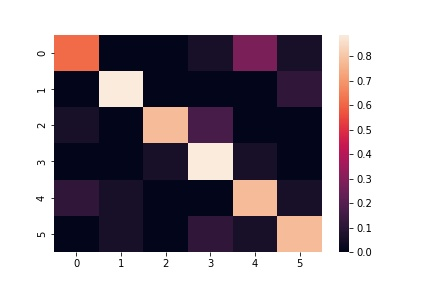
\includegraphics[width=\linewidth]{fedStanford901lr005_2x3others.jpg}
    \caption{Confusion matrix for FC layer}
  \end{subfigure}
  \begin{subfigure}[b]{0.4\linewidth}
    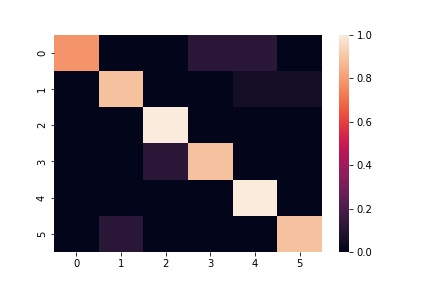
\includegraphics[width=\linewidth]{fedStanford901DA.jpg}
    \caption{Confusion matrix for LDA}
  \end{subfigure}
  \caption{Confusion matrix for FC layer and LDA}
  \label{fig:9FCLDA}
\end{figure}

As we explained the features we extract from images by using the frozen feature extractor can also be considered as the inputs. For that reason, what we had done by training a Resnet-18 with frozen feature extractor is same as training a single layer of fully connected layer with only inputs changing: images themselves for the former and the features of those images for the latter. This is an important point since there aren’t many techniques to train with image data yet there are many techniques when it comes to a training with a list of features. One such technique that we covered in EE573 was Linear Discriminant Analysis (LDA) and we decided to apply that technique to our task at hand. To do that we essentially followed the feature extraction we have just outlined. We extracted the features of all the data, fit our LDA classifier to training samples and then tested for the test set. We got 91\% accuracy with LDA. The confusion matrix can be seen at \ref{fig:9FCLDA}{(b)}. Since LDA work by finding axes that project good class separation, getting a good accuracy with LDA is a great sign of our feature extractor’s capacity to extract distinct features from different scenes and places.

The fact that LDA was the higher achiever of those two methods might seem a bit off but we should keep in mind since we frozen the feature extractor both LDA and the Fully Connected layer were getting the same inputs. So we only compared the stand alone performance of LDA and a single Fully Connected layer. So why did LDA outperformed the Fully Connected layer? After all they both are linear (We can only get nonlinearity in Deep Neural Networks by using nonlinear activation functions like ReLU between neural layers. The layers themselves and their combinations would otherwise always be linear.) We speculate accuracy discrepancy might indicate performance improvements with further training with smaller/decaying learning rate or maybe stacked fully connected layers might lead to improvements but doing so would require using a different training scheme or model architecture, respectively. 

One more thing we have noticed is in the previous test when the model predicted a wrong place, it was very likely it still predicted a place from the scene the label place belonged to. Like how it was predicting the wrong office but still an office. But now we see a lot of predictions that were not only the wrong place but also the wrong scene. We speculate this performance degradation is because our model was not trained and hence optimized for the feature space of these scenes. So, we are still using the features from previous scenes and when new features from different scenes resemble the same set of features from previous scenes the predictions might be off. 

\subsection{Effects of Dataset Diversity of Backbone's Adaptation to Novel Scenes}

	We have shown when we train a feature extractor with federated learning, we can use that feature extractor as frozen backbone of other client models that has completely different scenes. It is intuitive we will have better performance with such clients if we train our feature extractor with a more diverse dataset since that enables learning more features. We wanted to show that is indeed the case. To achieve that we have deployed a new federated learning scheme that’s nearly same as the previous one with the one exception: we removed the hallway places from the dataset. So, our dataset now consists of three offices and three lobbies. We have trained our model in federated setting with the exact same parameters using this new dataset. We have achieved 82\% accuracy in our test set which is an improvement over the 76\% we got last time. Yet last time we were classifying 9 places and we are now classifying 6. So, this improvement shall be considered with that in mind.
	
	
\begin{figure}[h!]
  \centering
  \begin{subfigure}[b]{0.4\linewidth}
    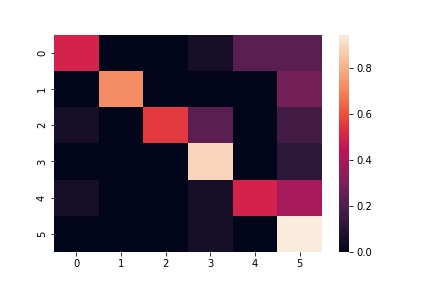
\includegraphics[width=\linewidth]{fedStanford601lr005_2x3others.jpg}
    \caption{Confusion matrix for FC layer}
  \end{subfigure}
  \begin{subfigure}[b]{0.4\linewidth}
    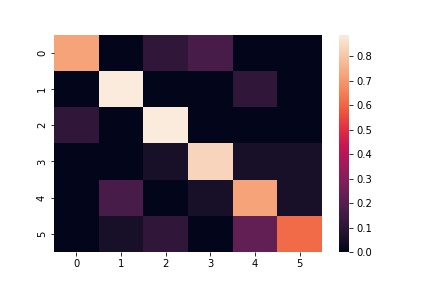
\includegraphics[width=\linewidth]{fedStanford601LDA.jpg}
    \caption{Confusion matrix for LDA}
  \end{subfigure}
  \caption{Confusion matrix for FC layer and LDA}
  \label{fig:6FCLDA}
\end{figure}

After we finished training the feature extractor, we followed the same previous steps to train a Fully Connected layer and LDA. Confusion matrixes we got can be seen at \ref{fig:6FCLDA}{(a and b)}. The accuracy of Fully Connected layer was 62\% and LDA got 77\%, so LDA outperformed FC once again. As we predicted the accuracy fell when we used a feature extractor that was trained with less diverse dataset. One other observation is just how frequently we predicted the wrong scene. We again speculate this is because our feature extractor only knows features from 6 places and 2 scenes it was trained with. The FC layer and LDA are trying to assign patterns of these features to the new scenes, but they aren’t quite successful due to poor quality of feature extractor. So we conclude the more diverse training data we use for feature extractor, the more robust it becomes adapting at novel scenes. This means we can increase the adaptibilty of our feature extractor to novel clients by introducing more clients during training. This is a very promising premise for applying federated learning to intelligent agents tasks/problems.


\pagebreak

\section{Conclusion}
\subsection{Results}

\par In this work, we tackled the heterogeneous local data problem for scene recognition tasks in which we desire agents to learn the scenes they have no samples of in their local data. If each agent is restricted to its own local data then this task becomes impossible unless we have some kind of information sharing technique. We proposed using federated learning to solve this problem by treating each agent as a client and modelling a server that synchronized the communication rounds and ensured information sharing while adhering to data privacy. To be more specific we have shown:
\begin{enumerate}
  \item Federated learning can be used for both IID and non-IID data distributions. But if we have non-IID data it is for the best to ensure full client participation.
  \item Encoding can be an effective way to reduce communication costs. Increasing the client participation we increase our system's robustness to adverse effects of encoding which could be modeled as noise.
  \item Federated learning innately provide data privacy but to combat privacy leakage differential privacy can be used. Just like encoding, differential privacy can be modelled as noise its adverse effects can be countered by increasing client count.
  \item If we desire to learn distinguishing different places from same scene, it is essential to use higher quality images and a more capable neural network architecture. We have managed to do that with ResNet-18 combined with 160x160 images for both central and federated settings.
  \item We can train a backbone/feature extractor in federated setting and then use it for novel scenes. For adaptation to novel scenes, this backbone can be paired up with a FC layer forming essentially original architecture or with a classical pattern recognition technique like LDA. 
  \item The more clients and diverse dataset we use for the training of this backbone, the better it performs at adapting the novel scenes.
\end{enumerate}

\subsection{Feature Work}

\par In this work, we were contraint by the hardware we have used. Had this not been the case we would investigate further the effects of increased number of clients and more diverse dataset in the backbone's adaption to novel clients. This can be a point investigated in the feature work. Additionally how the inclusion of a specific scene to training dataset affects the adaptation of specific novel scenes can be investigated. Intuitively, we expect the improvement in the accuracy of a specific novel scene if we add a scene closer to it to the training set. Also, effects of combining encoding with differential privacy can be investigated.

\subsection{Realistic Constraints}

\par Federated learning training requires more training rounds than the central training and this becomes more evident as the dataset becomes more and more heterogeneous. This leads to longer training times and needing more capable hardware. Additionally we have conducted our experiments assuming all the clients hold the same number of data samples in their local datasets and each scene had the same number of samples. This is a common assumption in federated learning research yet when it comes to real world application this requires preprocessing from client side. 

\subsection{Impact}

\par As people care more and more about their data privacy, stronger laws get into effect to ensure this right is protected. Since federated learning innately protect data privacy by not communicating client data to any server or using it anywhere else other than the local client, federated learning has become a popular research topic. We believe it is important to extend and combine this fededrated learning research to real-world examples. By using a real-world dataset and modelling data distributions of intelligent agents we tried to achieve that goal. Additionally given the fact that we used places from scenes like office -a place many people would regard as personal- data privacy is utmost importance. As we have shown federated learning based models can provide this privacy! In the future this can be extended to roomba robots or house robots as they become more prevelant. For such robots, both fast adaptation and privacy would be necessary and our work sets an example how this can be achieved.

\section{Acknowledgments}

\par I thank Prof. Işıl Bozma and Prof. Özlem Durmaz İncel for their helpful comments and suggestions.

\pagebreak
%--/Paper--

\begin{thebibliography}{9}

\bibitem{originalFL}
McMahan et al., “Communication-Efficient Learning of Deep Networks from Decentralized Data”, Feb 2017

\bibitem{TFF}
https://www.tensorflow.org/federated

\bibitem{stanfordDataset}
Armeni et al.,” Joint 2D-3D-Semantic Data for Indoor Scene Understanding”, Jan 2017

\bibitem{dirichlet}
Hsu et al.,” Measuring the Effects of Non-Identical Data Distribution for Federated Visual Classification”, Sep 2019

\bibitem{clientSelection1}
Cho et al., “Client Selection in Federated Learning: Convergence Analysis and Power-of-Choice Selection Strategies”, Oct 2020

\bibitem{clientSelection2}
Nishi et al., “Learning Advanced Client Selection Strategy for Federated Learning”, July 2019

\bibitem{compression1}
Haddadpour et al. “Federated Learning with Compression: Unified Analysis and Sharp Guarantees” Nov 2020

\bibitem{compression2}
Konecny et al., “FEDERATED LEARNING: STRATEGIES FOR IMPROVING COMMUNICATION EFFICIENCY”, Oct 2017

\bibitem{HE}
Madi et al., “A Secure Federated Learning framework using Homomorphic Encryption and Verifiable Computing” May 2021

\bibitem{SMC}
Truex et al., “A Hybrid Approach to Privacy-Preserving Federated Learning”, Aug 2019

\bibitem{diff1}
Abadi et al., "Deep Learning with Differential Privacy", Jul 2016

\bibitem{diff2}
McMahan et al., "Learning Differentially Private Recurrent Language Models", Oct 2017

\bibitem{resnet18}
He et al.,"Deep Residual Learning for Image Recognition", Dec 2015

\bibitem{advancesAndOpenProblems}
Kairouz et al.,"Advances and Open Problems in Federated Learning", Mar 2021

\bibitem{layerSharing}
Arivazhagan et al.,"Federated Learning with Personalization Layers", Dec 2019

\end{thebibliography}

\end{document}